\begin{figure}
  \centering
  \vspace*{-0.5cm}
  \begin{tikzpicture}
    \node at (0, 0){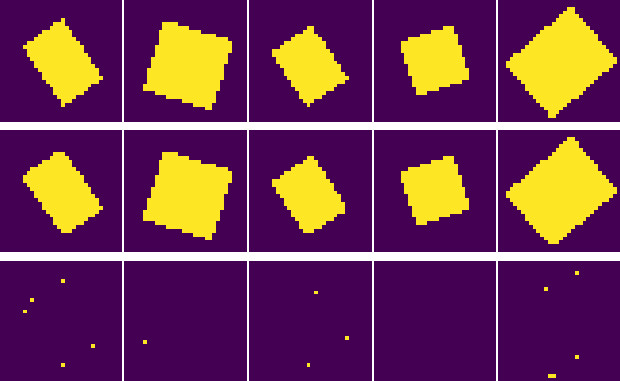
\includegraphics[width=5cm]{experiments/2d/vae_occ/easy_5/results_226000}};
    \node at (0, -4.25){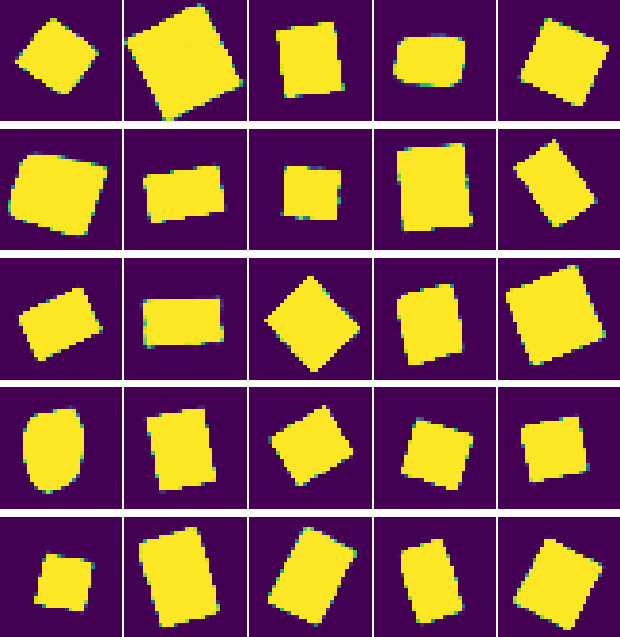
\includegraphics[width=5cm]{experiments/2d/vae_occ/easy_5/random_226000}};    
    \draw[-,dashed] (2.75, -13.25) -- (2.75, 1.5);
    
    \node at (5.5, 0){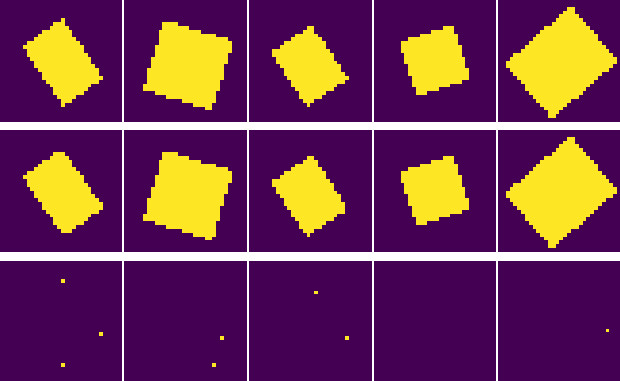
\includegraphics[width=5cm]{experiments/2d/vae_occ/easy_25/results_245000}};
    \node at (5.5, -4.25){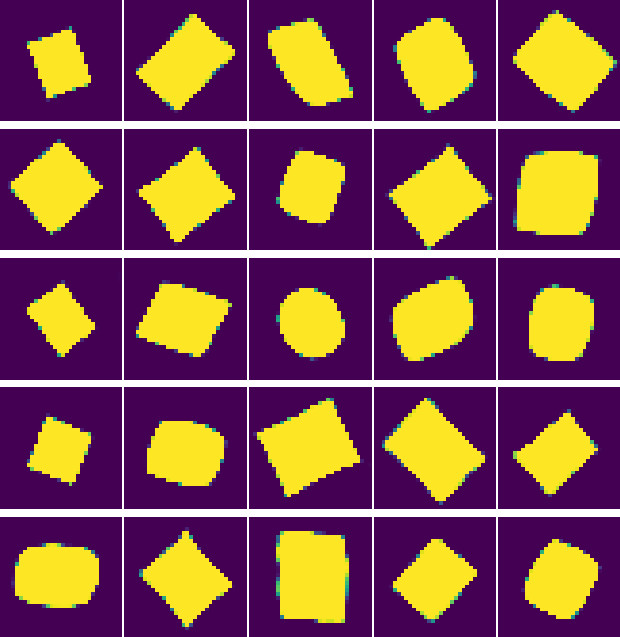
\includegraphics[width=5cm]{experiments/2d/vae_occ/easy_25/random_245000}};
   
    \node at (0, 2.25) {\begin{tabular}{c}$Q = 5$\\occupancy\end{tabular}};
    \node at (5.5, 2.25) {\begin{tabular}{c}$Q = 25$\\occupancy\end{tabular}};
    
    \node at (8.5,-4.25) {
      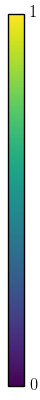
\includegraphics[height=5.5cm]{experiments/2d/ppca_occ/colorbar2}
    };
    
    \draw[-,dashed] (-2.75,-7) -- (8.5,-7);
    
    \node at (0, -9.75){
      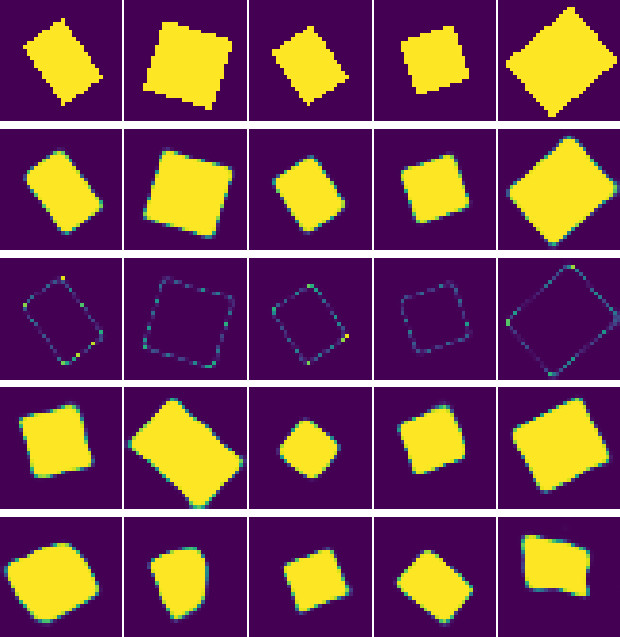
\includegraphics[width=5cm]{experiments/2d/vae_occ_sdf/easy_5_long/results_0}
    };    
    \draw[-,dashed] (2.75, -2.75) -- (2.75, 3);
    
    \node at (5.5, -9.75){
      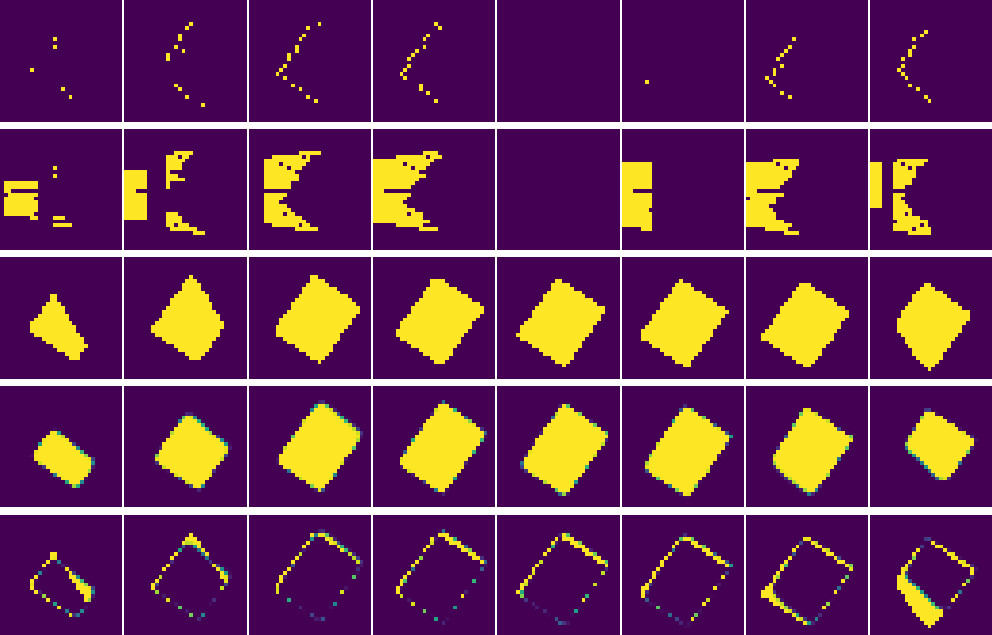
\includegraphics[width=5cm]{experiments/2d/vae_occ_sdf/easy_5_long/results_1}
    };
    \node at (8.5,-9.75) {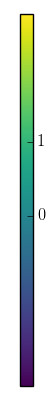
\includegraphics[height=5.5cm]{experiments/2d/vae_occ_sdf/easy_5_long/colorbar_1}};
   
    \node at (0, -13.25) {\begin{tabular}{c}$Q = 5$\\occupancy\end{tabular}};
    \node at (5.5, -13.25) {\begin{tabular}{c}$Q = 5$\\signed distance functions\end{tabular}};
    
    \node[rotate=90] at (-3.5, -3) {\begin{tabular}{c}predicting occupancy only\end{tabular}};
    \node[rotate=90] at (-3.5, -9.75) {\begin{tabular}{c}predicting occupancy and\\signed distance functions\end{tabular}};
  \end{tikzpicture}
  \vskip 6px
  
  % TODO short caption
  \caption{A comparison of random samples for \VAE shape rpiors using $Q = 5$
  and $Q = 25$ for occupancy only
  (top) and $Q = 5$ for occupancy and signed distance functions (bottom).
  In the former case, we show reconstructions of five samples for $Q = 5$
  and $Q = 25$, respectively, illustrating target shape in the first row,
  followed by the prediction and its error. Below we show $25$ random samples.
  For the latter case, we show the target shapes in the first row,
  the reconstruction and the corresponding error
  in the next two rows and, finally, two rows of random samples.}
  \label{fig:experiments-2d-vae-occ-random}
\end{figure}
